\documentclass[10pt,a4paper]{article}
\usepackage[margin=2.2cm]{geometry}
\usepackage{fontspec}
\usepackage{kotex}
\setmainfont{Apple SD Gothic Neo}
\setsansfont{Apple SD Gothic Neo}
\usepackage{amsmath,amssymb}
\usepackage{graphicx}
\usepackage{booktabs}
\usepackage{caption}
\usepackage[dvipsnames]{xcolor}
\usepackage[colorlinks=true,linkcolor=MidnightBlue,citecolor=MidnightBlue,
            urlcolor=MidnightBlue]{hyperref}
\usepackage{titlesec}
\titleformat{\section}{\large\bfseries}{\thesection}{0.6em}{}
\titleformat{\subsection}{\normalsize\bfseries}{\thesubsection}{0.5em}{}
\captionsetup{font=small,labelfont=bf}
\setlength{\parskip}{0.35em}
\setlength{\parindent}{0pt}

\usepackage{mdframed}
\newmdenv[linewidth=0.4pt,linecolor=gray!60,backgroundcolor=gray!5,
          innertopmargin=6pt,innerbottommargin=6pt,skipabove=8pt,skipbelow=8pt]{claimbox}
\newcommand{\claim}[2]{\begin{claimbox}\textbf{주장.} #1\par\smallskip
  \textcolor{gray!70}{\textbf{반증 조건.} #2}\end{claimbox}}

\title{\bfseries 고치니 더 뚜렷해졌다\\[2pt]
\large 공통 비용이 신호 몫을 희석하고 있었다 --- 그리고 방향 뒤집힘은 기제가 아니었다}
\author{월드모델 실험실 · 노트 753 $\sim$ 757}
\date{2026-08-07}
\begin{document}\maketitle

\section{한 줄}

논문 $147$ 이 \textbf{축이 유보보다 먼저 끝나면 판 비용이 $4.2$배}($13.8\sigma$)임을
쟀고, 그것이 장 시간축 실험의 순효과 $-0.0434$ 중 $0.0308$ 을 설명했다. 그래서
\textbf{그 구멍을 메우고 다시 쟀다.}

\textbf{위약 비용이 $0.0302 \to 0.0092$ 로 $70\%$ 줄었다.} 그런데 \textbf{신호 몫이
$-0.0132 \to \mathbf{-0.0192}$ 로 더 음수가 됐다.} 예측과 반대다 --- 그리고 그 반대가
발견이다: \textbf{두 팔에 공통으로 실린 비용은 차이를 $0$ 쪽으로 당긴다.}

\section{구멍을 메운 방법 --- 유보를 자르지 않고 앞채움}

논문 $147$ 이 처방 둘을 적었다: \textbf{유보를 축의 관측 끝까지로 자르거나, 유보 끝까지
덮는 축만 쓰거나.} \textbf{셋째 길을 골랐다} --- 판 행 날짜가 장의 끝($2026.51$)을
넘으면 \textbf{장의 마지막 관측값}을 쓴다.

\begin{center}
\begin{tabular}{ll}
\toprule
① & \textbf{판을 그대로 두므로} 논문 $147$ 의 값과 직접 비교된다(유보를 자르면 분모가 바뀐다) \\
② & \textbf{예보 시점에 관측 가능하다} --- $2026.8$ 행을 채점할 때 $2026.51$ 관측은 이미 있다 \\
③ & \textbf{배포에서 실제로 하는 일이다} --- 자료는 늘 며칠 늦다 \\
\bottomrule
\end{tabular}
\end{center}

\textbf{배선 검사: 유보 덮음률 $\mathbf{1.000}$ --- $11$ 도메인 전부.} 아래 경계
($2020.15$)는 학습 구간 안이므로 유보 전체가 그 뒤다.

\begin{figure}[t]\centering
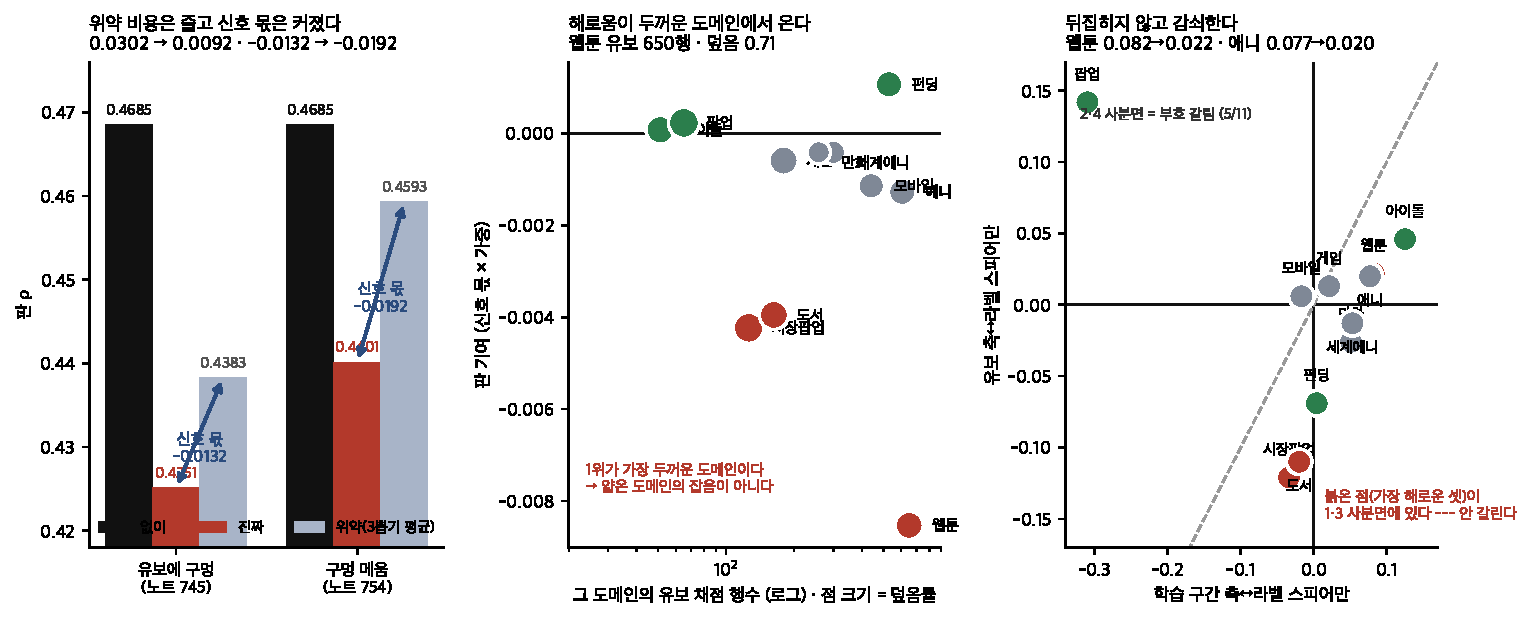
\includegraphics[width=0.99\textwidth]{figs/dilution.pdf}
\caption{왼쪽: \textbf{위약 비용은 줄고 신호 몫은 커졌다.} 가운데: \textbf{해로움이
가장 두꺼운 도메인에서 온다} --- 판 기여 $1$위 웹툰은 유보 $650$행이다. 오른쪽:
\textbf{뒤집히지 않고 감쇠한다} --- 붉은 점(가장 해로운 셋)이 $1 \cdot 3$ 사분면에 있다.}
\end{figure}

\section{결과 --- 노트 745 가 확정됐다}

\begin{center}
\begin{tabular}{lrrl}
\toprule
& 유보에 구멍(노트 $745$) & \textbf{구멍 메움} & \\
\midrule
없이 & $0.4685$ & $0.4685$ & 같다 \\
진짜 & $0.4251$ & $\mathbf{0.4401}$ & 올라왔다 \\
위약 $3$뽑기 평균 & $0.4383$ & $0.4593$ & 올라왔다 \\
\midrule
\textbf{위약 비용} & $0.0302$ & $\mathbf{0.0092}$ & \textbf{$70\%$ 줄었다} \\
순효과 & $-0.0434$ & $-0.0284$ & 덜 나빠졌다 \\
\textbf{신호 몫} & $-0.0132$ & $\mathbf{-0.0192}$ & \textbf{더 음수다} \\
팝업 · 시장팝업 뺀 신호 몫 & $-0.0090$ & $-0.0160$ & \\
\bottomrule
\end{tabular}
\end{center}

신호 몫 $-0.0192$ 는 판 문턱($0.0045$)의 \textbf{$4.3$배 음수}다. 위약 뽑기 SD
$0.0032$ · 순효과 짝 SD $0.0019$. \textbf{사전등록 규칙 (가) 발동 --- 확정이다.}

\claim{\textbf{공통 비용은 신호 몫을 희석한다. 그래서 배선을 고치면 효과 크기가
\emph{커질} 수 있다.} 마스크 비용 $0.0302$ 는 진짜와 위약에 \textbf{공통으로} 실려
있었고, 판이 이미 $0.03$ 내려간 자리에서는 열 하나가 더 나빠질 여지가 줄어든다(바닥
효과). \textbf{그러므로 배선이 나쁜 상태에서 잰 음수도, 양수도 과소평가일 수 있다} ---
``배선이 나쁘면 효과가 안 보인다''의 반대쪽이다.}
{바닥 효과가 아니라 \textbf{마스크가 실제로 신호를 나르고 있었을} 수도 있다 --- 구멍이
있을 때 진짜 팔의 마스크가 ``$2026.51$ 이후''를 표시하므로 그 자체가 시간 정보다. 그러면
진짜 팔이 그 정보로 조금 덜 나빠졌던 것이고, 메우니 그 도움이 사라진 것이다.
\textbf{두 설명을 이 실험은 못 가른다} --- 가르려면 마스크를 무작위로 같은 비율만큼
비워야 한다. 안 했다.}

\subsection*{해로움이 얇은 도메인의 잡음이 아니다}

\begin{center}
\begin{tabular}{lrrr|lrrr}
\toprule
도메인 & 판 기여 & 유보 & 덮음 & 도메인 & 판 기여 & 유보 & 덮음 \\
\midrule
\textbf{웹툰} & $\mathbf{-0.00853}$ & $650$ & $0.71$ & 게임 & $-0.00059$ & $180$ & $0.83$ \\
시장팝업 & $-0.00423$ & $126$ & $1.00$ & 세계애니 & $-0.00041$ & $300$ & $0.36$ \\
도서 & $-0.00395$ & $163$ & $0.81$ & 만화 & $-0.00041$ & $258$ & $0.27$ \\
애니 & $-0.00127$ & $606$ & $0.64$ & 아이돌 & $+0.00008$ & $51$ & $0.76$ \\
모바일 & $-0.00114$ & $441$ & $0.55$ & 팝업 & $+0.00023$ & $65$ & $1.00$ \\
& & & & 펀딩 & $+0.00107$ & $529$ & $0.66$ \\
\bottomrule
\end{tabular}
\end{center}

\textbf{$1$위가 웹툰이다} --- 유보 $650$행으로 가장 두껍고 덮음 $0.71$ 이며, 논문 $146$
의 잡음 배수기 목록에서 \textbf{가장 안 흔들리는} 도메인이었다(순수 난수 $3$열이
$+0.0043$). 규약 $19$(유보 행수와 잡음 민감도를 같이 적는다)를 지켜 적는다 ---
\textbf{이 음수는 시장팝업 탓이 아니다.}

\section{왜 해로운가 --- 방향 뒤집힘은 아니다}

가장 그럴듯한 기제는 \textbf{방향 뒤집힘}이었다: 축과 라벨의 관계가 학습과 유보에서
부호가 다르면 판이 학습에서 배운 것을 유보에서 거꾸로 쓴다(노트 $604$ 계열 · 입문서
$04$면이 이미 잰 기제). \textbf{판을 안 적합하고 잴 수 있어서 쟀다.}

\begin{center}
\begin{tabular}{lrrcl}
\toprule
도메인 & 학습 상관 & 유보 상관 & 갈림 & 판 기여 \\
\midrule
\textbf{웹툰} & $+0.082$ & $+0.022$ & \textbf{아니오} & $-0.00853$ \\
시장팝업 & $-0.034$ & $-0.121$ & \textbf{아니오} & $-0.00423$ \\
\textbf{도서} & $-0.020$ & $-0.110$ & \textbf{아니오} & $-0.00395$ \\
애니 & $+0.077$ & $+0.020$ & \textbf{아니오} & $-0.00127$ \\
모바일 & $-0.017$ & $+0.006$ & 예 & $-0.00114$ \\
만화 & $+0.051$ & $-0.026$ & 예 & $-0.00041$ \\
세계애니 & $+0.053$ & $-0.013$ & 예 & $-0.00041$ \\
팝업 & $-0.310$ & $+0.142$ & 예 & $+0.00023$ \\
펀딩 & $+0.004$ & $-0.069$ & 예 & $+0.00107$ \\
\bottomrule
\end{tabular}
\end{center}

\textbf{부호 갈림 $5/11$ 이고 가장 해로운 둘(웹툰 · 도서)이 안 갈린다.} 게다가
\textbf{갈림 $\leftrightarrow$ 판 기여 스피어만이 $+0.637$} 이다 --- \textbf{갈리는
도메인이 오히려 덜 해롭다.} 예측 둘이 함께 반증됐다.

\claim{\textbf{뒤집히지 않고 감쇠한다.} 가장 해로운 둘의 무늬가 같다 --- 웹툰
$+0.082 \to +0.022$ · 애니 $+0.077 \to +0.020$ 로 \textbf{부호가 아니라 크기가
$4$분의 $1$로 준다.} 그러면 기제 후보는 \textbf{약한 신호가 강한 분할 여지를
준다}는 것이다: 이 축은 날짜에서 왔으므로 고유값이 많은데(웹툰 $1{,}594$) 관계가
$0.08$ 밖에 안 되므로 \textbf{쪼갠 것 대부분이 잡음 적합}이다.}
{전수로는 안 맞는다 --- \textbf{도서 · 시장팝업은 유보에서 오히려 강해진다}
($-0.020 \to -0.110$ · $-0.034 \to -0.121$). 다만 그 둘의 학습 행이 $34 \cdot 123$
으로 얇아 \textbf{학습 상관 자체가 잡음}이다. \textbf{그리고 이 기제는 안 쟀다} ---
축을 거칠게 만들어(고유값 $10 \cdot 4$) 해로움이 줄면 기제가 서고, 그것이 동시에
고침이다. 그 측정을 다음으로 등록했다.}

\section{내 사전등록에 구멍이 있었다}

\claim{\textbf{사전등록 규칙은 값의 전 구간을 덮어야 한다.} 방향 실험의 규칙을
\emph{``갈림 $\geq 6/11$ 이면 (가) · $\leq 4$ 이면 (나)''}로 적었고 \textbf{실측이
$5$ 다} --- \textbf{어느 쪽도 발동하지 않는다.} 구멍이 있으면 \textbf{결과를 보고
규칙을 고르게 되고}, 그것이 사전등록을 무너뜨린다.}
{규칙을 촘촘히 적으면 읽기 어려워진다는 반론이 있다. 그러나 \textbf{경계를
$\geq 5$ / $< 5$ 로 붙여 쓰면 길이가 그대로다} --- 구멍은 표현의 문제가 아니라
\textbf{내가 그 값이 나올 줄 몰랐다는 표시}다.}

\subsection*{그리고 같은 실수를 두 번 했다 --- 최댓값을 자로 썼다}

논문 $147$ 의 결측 실험에서 \textbf{최대 뽑기 SD}($0.0034$ · 유난히 흔들린 팔에서 왔다)를
자로 써서 ``셋이 비슷''이 형식상 발동했다. 이번 방향 실험에서도 \textbf{학습 $|$상관$|$
최대}($0.310$ · 학습 $24$행인 팝업)로 규칙 (다)가 발동했다 --- \textbf{중앙값은
$0.051$} 이다.

\begin{center}
\textbf{자는 최댓값이 아니라 중앙값이나 \emph{비교하는 두 항}의 잡음으로 만든다.}\\
최댓값을 쓰면 \textbf{가장 얇은 도메인이 자를 정한다.}
\end{center}

\section{그래서 T2 의 통로 ②를 닫는다}

\claim{\textbf{장의 전국 시간축은 판을 해친다 --- 확정.} 문턱의 $4.3$배 음수 · 위약
$3$ 뽑기 · 마스크 결함을 고친 뒤 · 팝업 둘을 빼도 $-0.0160$ · 판 기여 $1$위가 가장
두꺼운 도메인. \textbf{L2 를 판으로 옮기는 통로 둘이 다 닫혔다}: ① 동네를 붙이는 길
(판의 $1.5\%$ · 노트 $646$) ② 전국 시간축(여기). \textbf{세 번째 길만 남았다} ---
IP 에 지역을 붙일 수 있는 자료.}
{\textbf{이 축은 전국 하나의 수}라 장의 동네별 정보를 전부 버렸다. \textbf{실패가
``장은 쓸모없다''를 뜻하지 않는다} --- 장 자신의 과제에서는 지속성을 이긴다(논문
$145$ · 유보 $R^2$ $+0.1200$ · $5.6\sigma$). \textbf{그리고 다음 실험이 이 결론을
좁힐 수 있다} --- 축을 거칠게 해서 해로움이 사라지면 ``이 축은 못 쓴다''가
``이 해상도로는 못 쓴다''가 된다.}

\end{document}
